\section{Experiment Process and Results}

\subsection{Phase 1: Codex Incremental Build---Attempt and Stagnation}

In Phase~1, Codex was used with the Incremental Build strategy. The AI was first prompted to construct a page skeleton (HTML structure plus basic CSS), then a splash screen animation and background image were added. The plan was to gradually add content modules---self-introduction, data visualization, and easter eggs---on top of this foundation.

However, even at this earliest stage, a palpable sense of disempowerment set in. Although every element had been added through the user's own prompts, there was no clear vision of what the final page should look like---the skeleton itself resembled a generic template, neither aesthetically pleasing nor personally distinctive. Continuing in this mode would mean relying on each subsequent module's prompt to precisely hit a vaguely imagined target, which was clearly unrealistic.

The entire process halted at a very early stage: build skeleton $\rightarrow$ add splash screen animation $\rightarrow$ add background $\rightarrow$ feel a lack of direction $\rightarrow$ \textbf{stagnation}.

\begin{figure}[t]
\centering
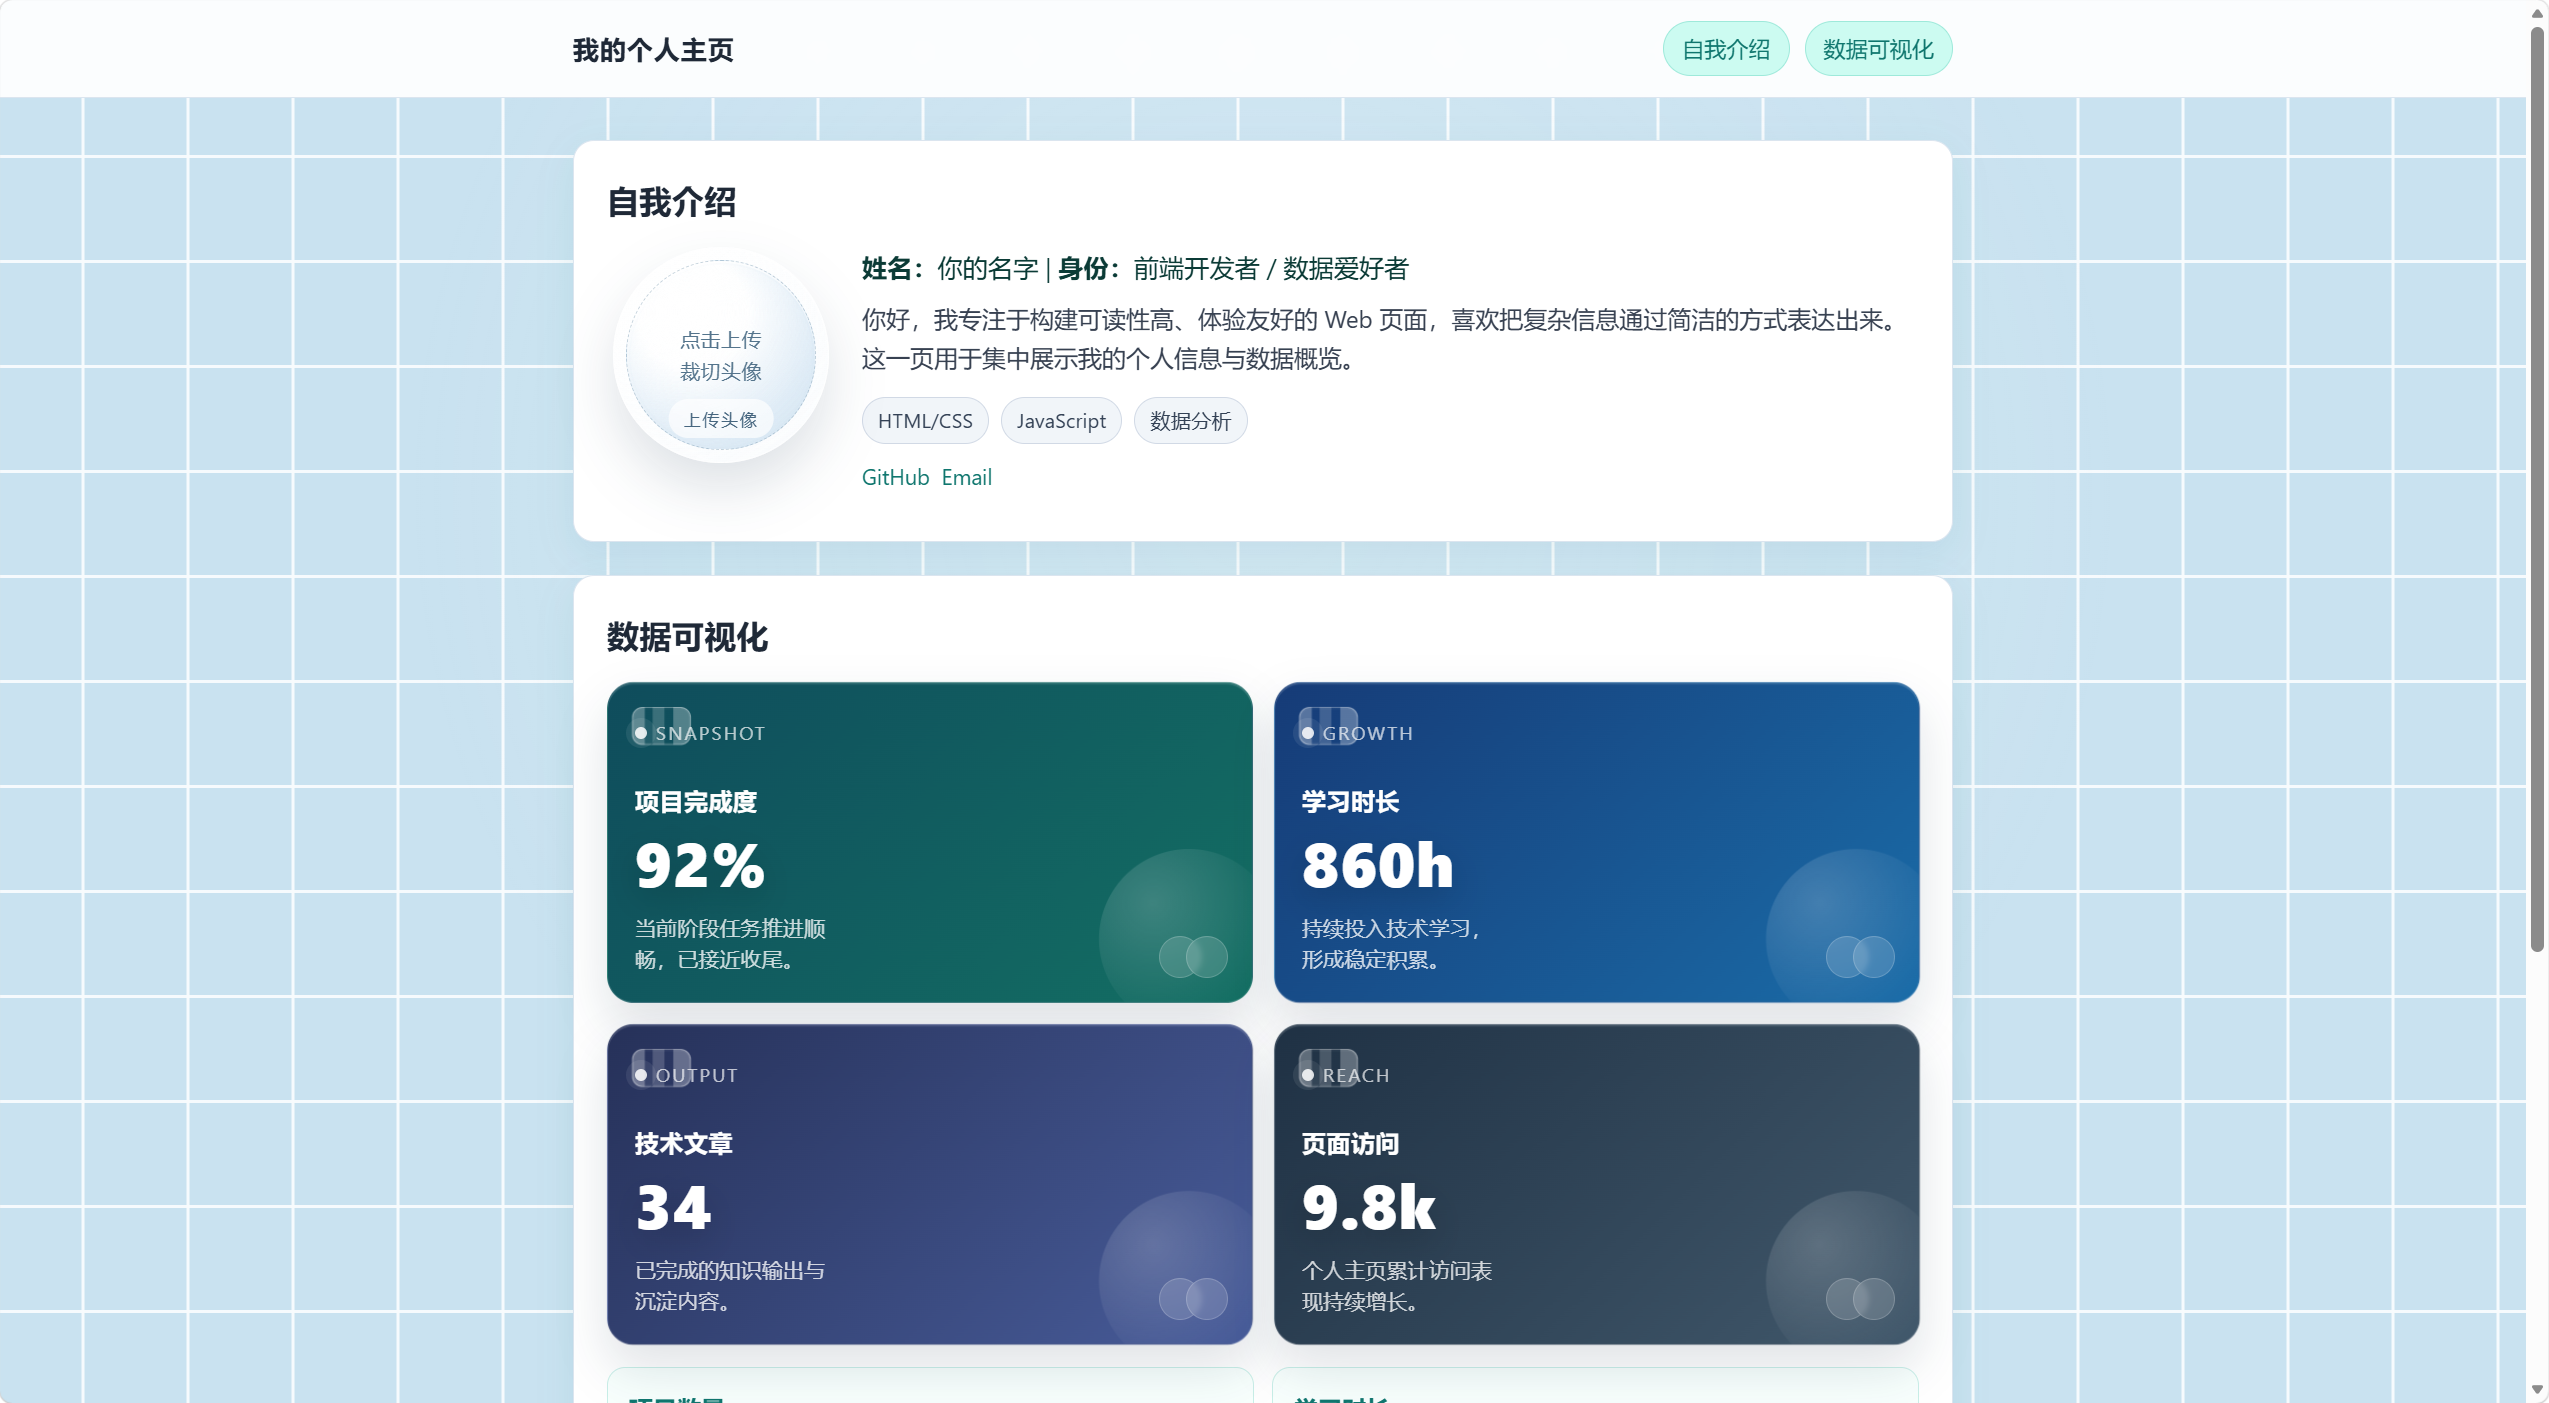
\includegraphics[width=0.85\linewidth]{../图片/第一版首页截图.png}
\caption{Codex Phase~1 homepage result: only a skeleton, a splash animation, and a background image, lacking design identity and a unified visual language.}
\label{fig:codex}
\end{figure}

Analyzing the cause of failure, the core problem was \textit{the absence of any design anchor}. The initial prompt was a vague description along the lines of ``help me make a personal homepage''---the AI dutifully completed the instruction, but it produced \textit{anyone's} homepage, not \textit{mine}. Without first establishing a design direction (color palette, typography, aesthetic tone, animation principles), each prompt operated in isolation with no shared reference.
Although the process terminated prematurely and never reached the stage of ``multi-module style conflict,'' the experience at that point already allowed two predictions: first, each subsequent module would require extremely precise prompts to match a fuzzy mental image---nearly impossible for a non-expert user; second, even if individual modules were adjusted to an acceptable level through separate prompts, without a unified design document, they would inevitably clash when assembled together.

\subsection{Phase 2: Claude Code Design-First---Complete Implementation}

Learning from Phase~1, Claude Code was adopted with a fundamentally different strategy: invest substantial time in discussing and finalizing the design with the AI before writing any code. Approximately 20\% of the total dialogue rounds were spent on pre-coding design discussion.

\textbf{Design Philosophy.} The first step of Phase~2 was not ``write code'' but ``discuss the feel.'' The AI initially proposed a ``warmth''-oriented direction with a warm color palette, paper texture, and serif typography. The user supplemented this with a ``sharpness'' dimension---precision in animation and attention to detail in interaction, avoiding excessive softness. The AI synthesized these into a contradiction framework: ``warmth is the material, sharpness is the craft''---the background feels like old book paper with generous whitespace, while animations are precise and restrained, and interactive details are crisp. A third keyword, ``vitality,'' was added later---particles drift, a vinyl record rotates, corner plants sway in a gentle breeze. The page should not feel like a static display board.

\begin{figure}[t]
\centering

\includegraphics[width=0.85\linewidth]{../图片/第二版首屏.png}
\caption{Phase~2 hero section: staggered character drop animation, diamond decorative lines, warm glow following the cursor, floating particles.}
\label{fig:v2-hero}
\end{figure}

\textbf{Final Deliverable.} The final implementation is a complete single-page website with six regions, deployed via GitHub Pages (URL: \url{https://qaq82625.github.io/-v2.0/}). The codebase totals approximately 3,700 lines (HTML:~470 lines, CSS:~3,100 lines, JavaScript:~1,700 lines), produced over roughly 200 dialogue rounds.

\begin{figure}[t]
\centering
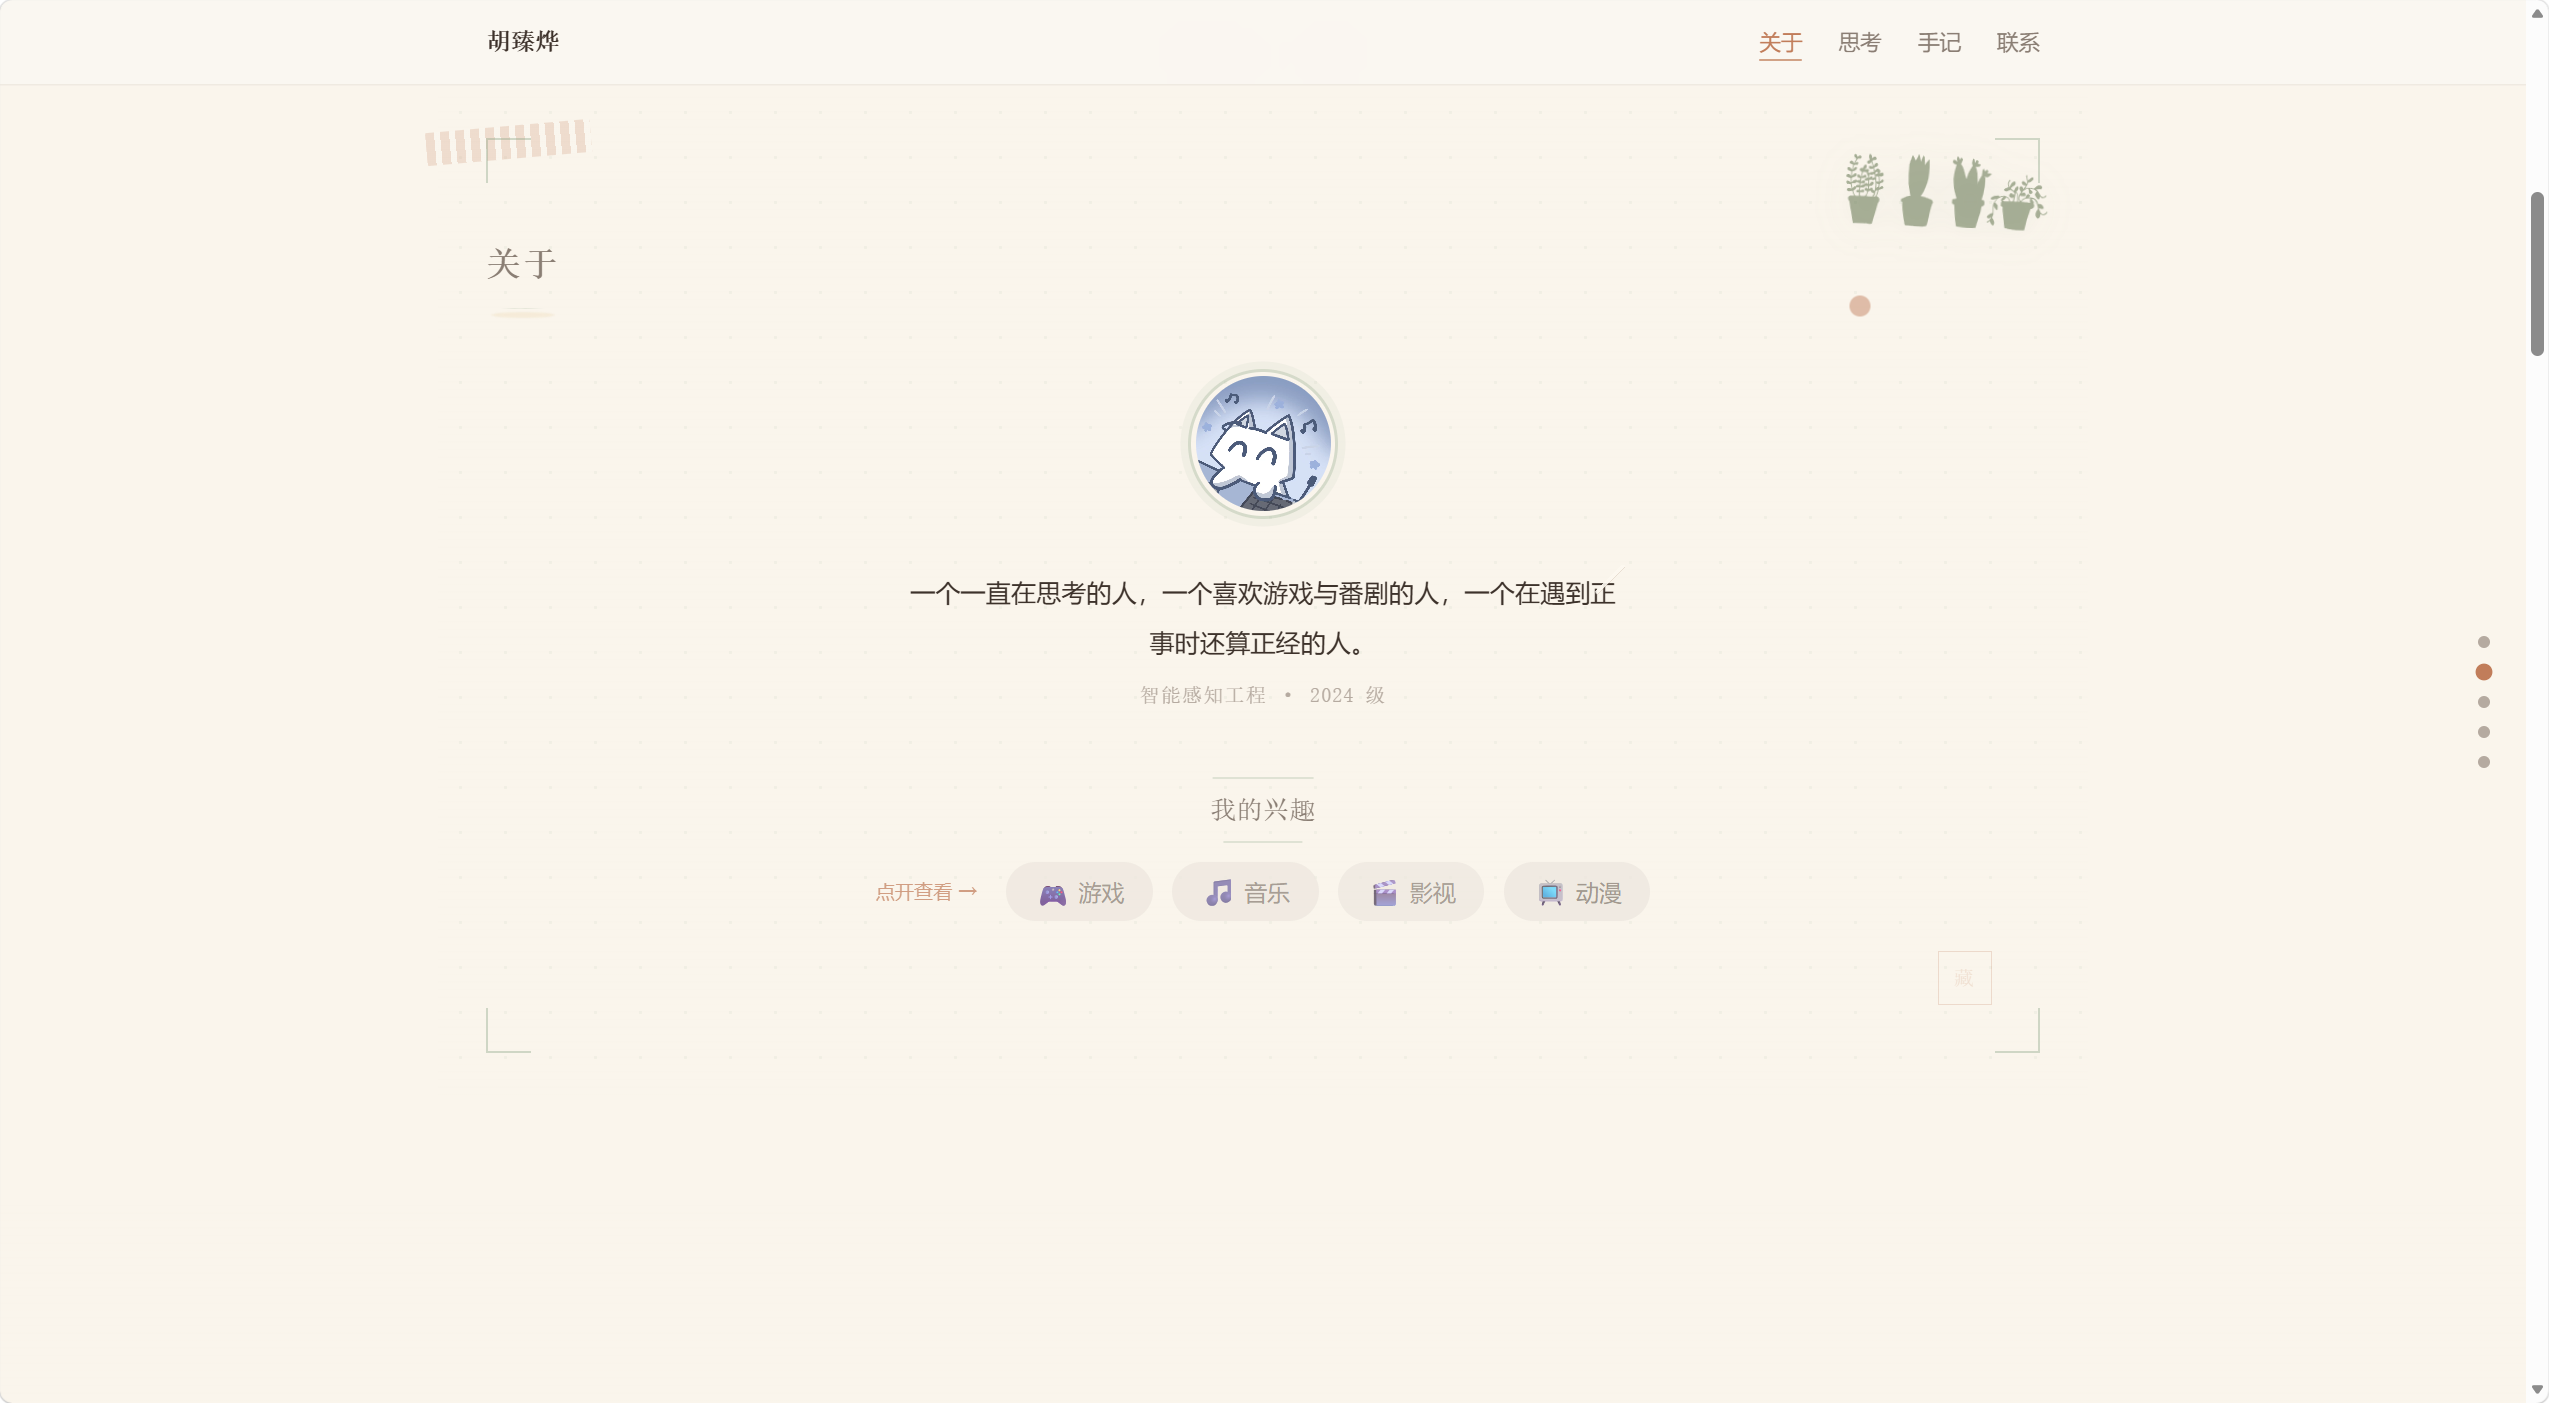
\includegraphics[width=0.85\linewidth]{../图片/关于页界面.png}
\caption{About section: avatar, self-introduction, major and year, four interest tags (clickable to expand themed data visualization panels).}
\label{fig:about}
\end{figure}

\subsection{Core Features and Interactions}

\textbf{Data Visualization.} The four interest tags in the About section (Gaming, Music, Film, Anime) each correspond to an independently designed data panel. The user specified the visual direction for each tag during the design discussion---pixel art for gaming, vinyl record with sound waves for music, vintage ticket stub for film, CRT television for anime---and the AI implemented independent theme styles and bespoke animations for each. Specifically: the gaming panel adopts a retro cartridge slot style with a 200$\times$50px four-frame spritesheet for a walking character animation (50$\times$50px per frame, 350\,ms frame interval); the music panel uses CSS \texttt{conic-gradient} to render a rotating vinyl disc (8-second full rotation) with the current listening count displayed in handwriting font at the center, and 12 waveform bars that randomize their heights every 120\,ms; the film panel uses a vertical ticket stub layout with circular cutouts simulating perforated tear edges, film titles rendered in handwriting font, and a stamp-style tagline at the bottom; the anime panel simulates a CRT television appearance with scanline overlay and radial vignette on the screen area, recommendation text drifting from right to left in bullet-comment style (8-second cycle), and a star icon beside the title pulsing at a 1.5-second period. The four panels operate with mutually exclusive expansion logic---only one panel is shown at a time, clicking the same tag closes it, clicking outside the panel closes it, and clicking a different tag directly switches content.

\textbf{Horizontal Scroll (Signature Interaction).} The Thoughts section houses the homepage's core interaction. It uses GSAP ScrollTrigger's pin+scrub mechanism: as the visitor scrolls down the page, upon reaching the Thoughts section, vertical scrolling is ``captured'' and converted into horizontal displacement of the card track, with six article cards sliding through one by one. The centered card automatically receives a ``spotlight'' effect (scale: 1, opacity: 1), while flanking cards are automatically dimmed (scale: 0.94, opacity: 0.55), with smooth transitions. Each card contains a cover image, date, title, one-line summary, and tags. Below the card track are six navigation dots (the current card's dot is enlarged 1.5$\times$) and left/right arrows (auto-hidden at the first and last cards), with a position counter displayed at the bottom right (1/6 through 6/6). On mobile devices (below 640\,px), the interaction gracefully degrades to a normal vertical card layout, with the navigation indicator hidden.

\begin{figure}[t]
\centering
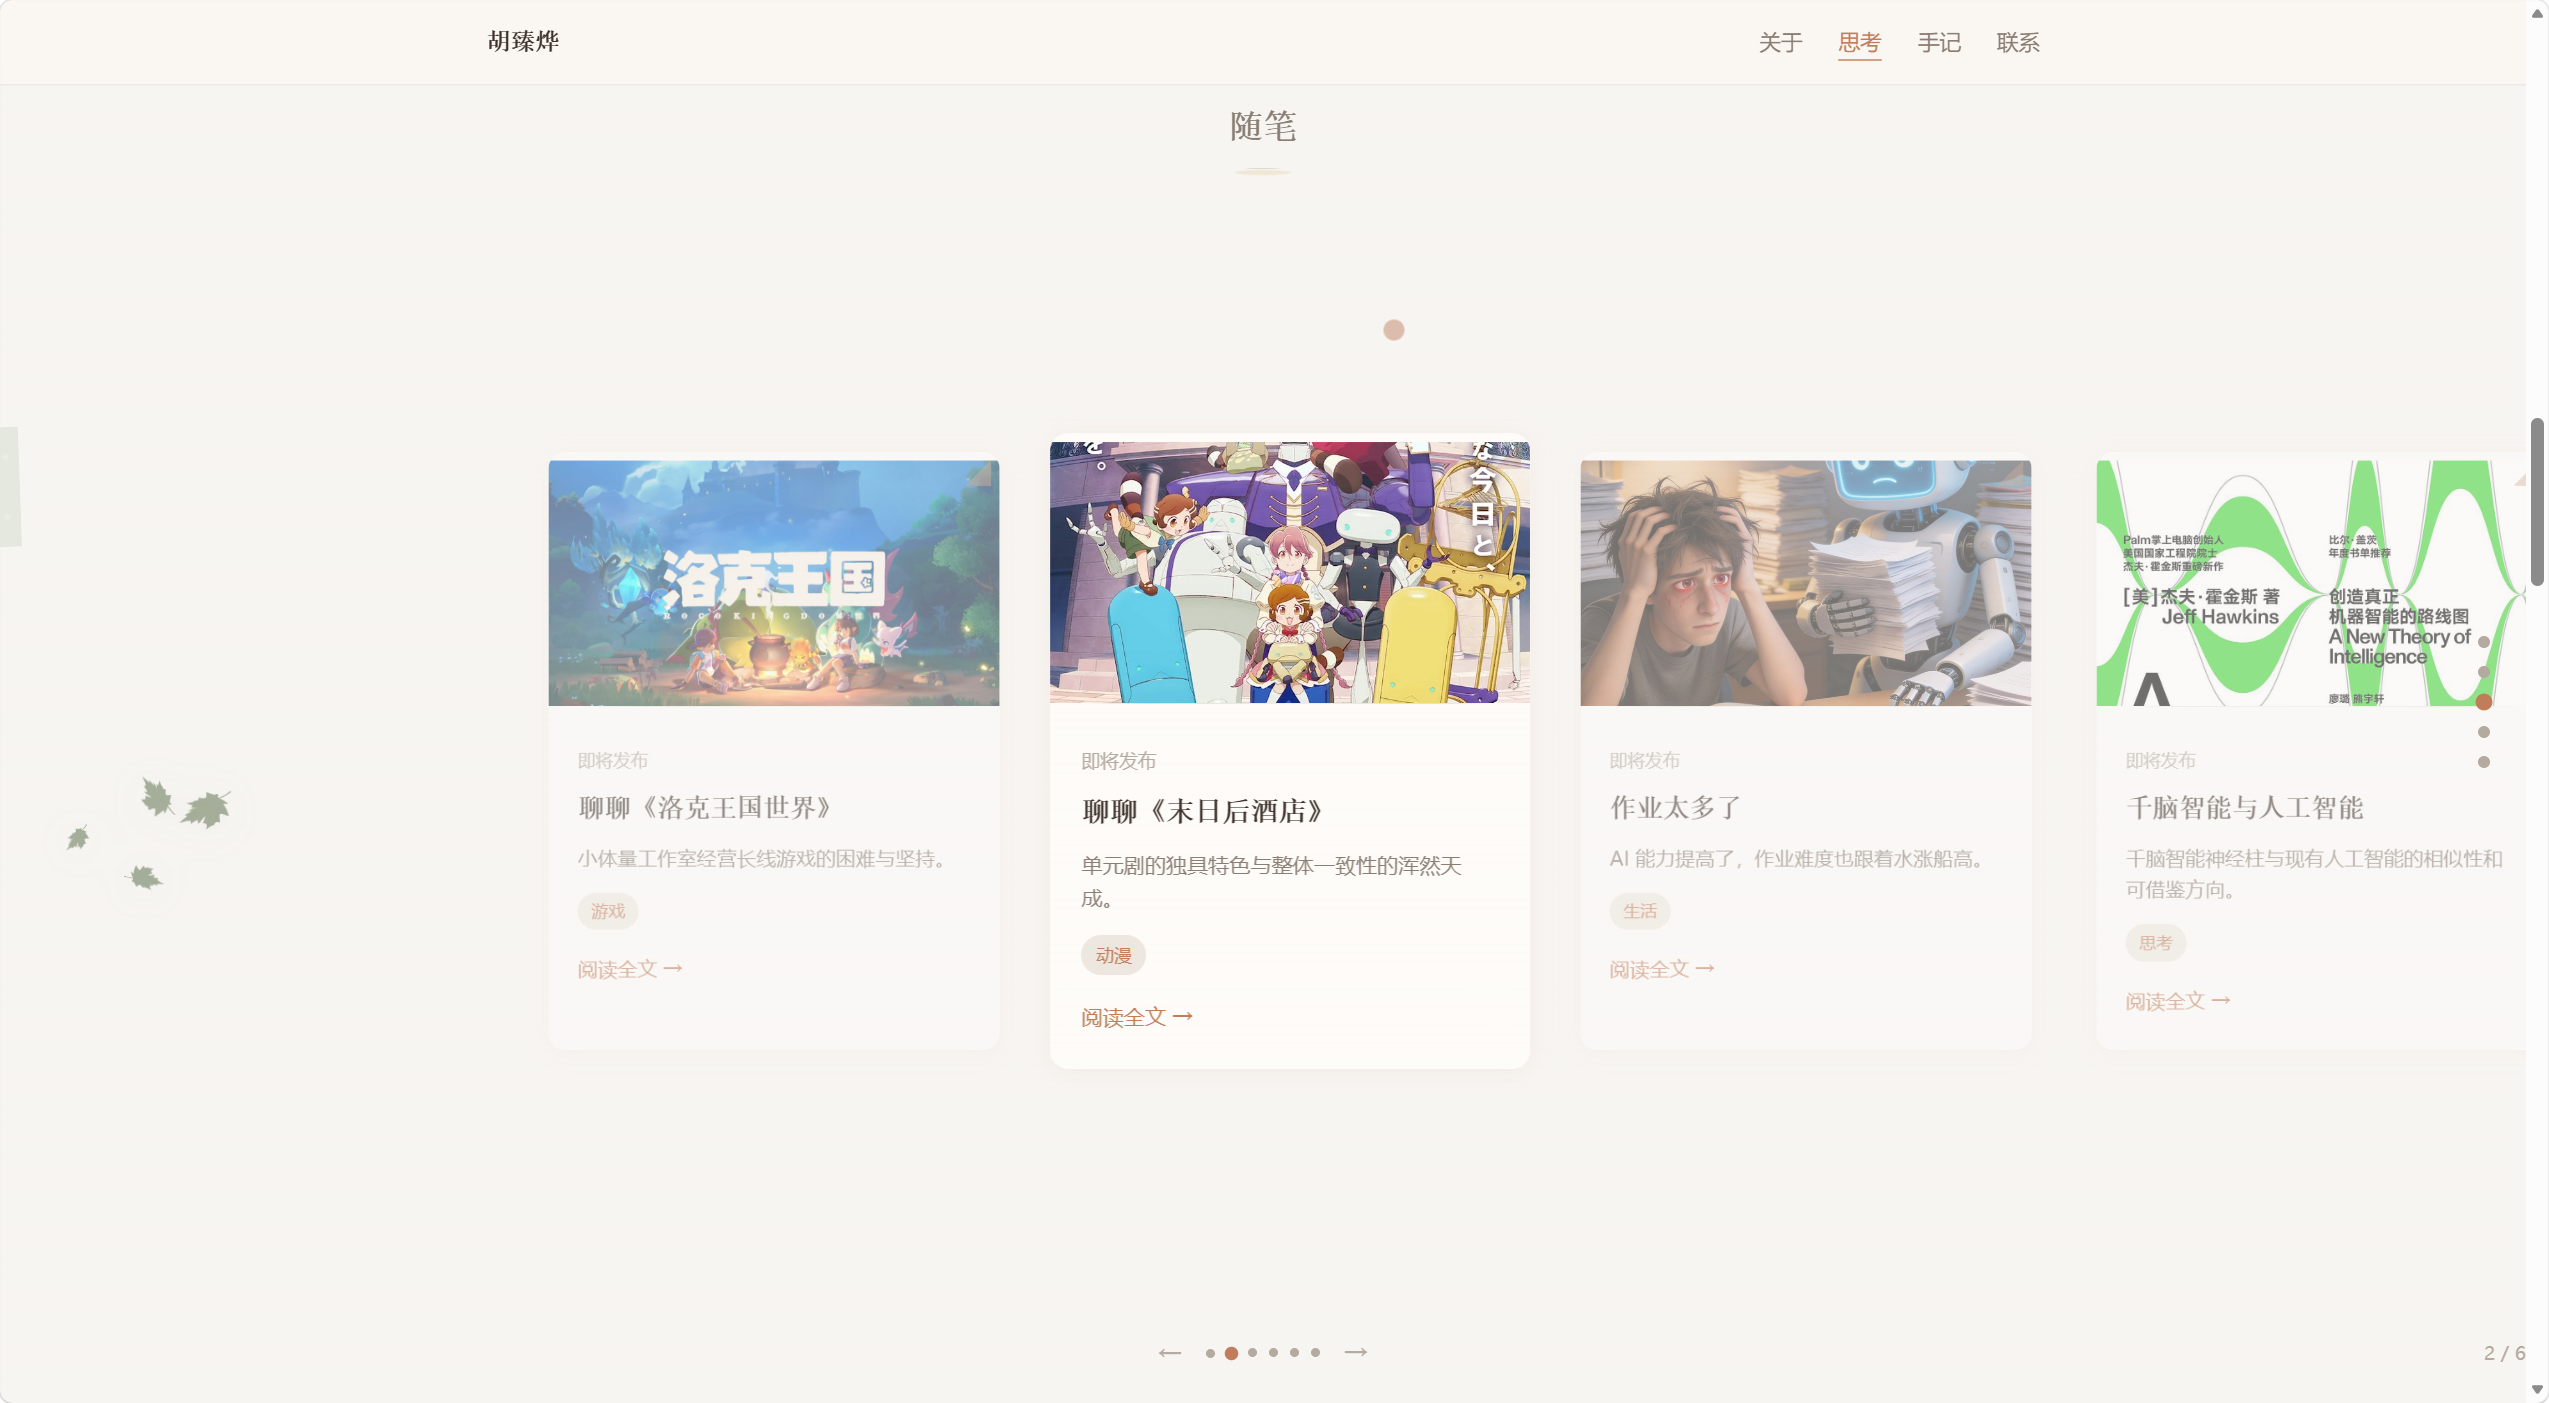
\includegraphics[width=0.85\linewidth]{../图片/思考区横向.png}
\caption{Thoughts section horizontal scroll: centered card with spotlight effect, dot navigation indicating current position (1/6).}
\label{fig:thoughts}
\end{figure}

\textbf{Easter Egg System.} The footer contains five easter eggs tiered by discovery difficulty: L1---Time-aware greeting (auto-displayed, switching among four greetings---morning/day/evening/night---based on \texttt{new Date().getHours()}); L2---Hidden playlist (click the music note icon to expand an HTML5 Audio mini-player with two embedded mp3 files; completing a full song automatically unlocks the ``Music Connoisseur'' achievement) and Achievement system (six badges with unlock conditions spanning Time Traveler, Music Connoisseur, Secret Reader, Note Leaver, Game Master, and Night Owl; unlocking triggers 14 colored confetti particles bursting from the screen center); L3---Hidden message (hovering on the copyright line for 1.5 seconds causes the text to dissolve via GSAP and reform as the secret message ``You even looked here---then we should be friends,'' reverting when the cursor moves away); L4---Snake mini-game (clicking the footer tilde ornament five times within 1.2 seconds triggers a full-screen Canvas game, 360$\times$360\,px arena with CELL~=~20\,px, snake body in terra-cotta gradient, food in sage green circles, subtle grid background, controlled via arrow keys / WASD / touch swipe, high score stored in localStorage); L5---Time preview clock (a clock button in the footer cycles through six time periods to preview the full-day atmosphere color shifts; switching updates CSS custom properties---\texttt{--bg}, \texttt{--bg-warm}, etc.---in real time, with glow color and greeting text responding synchronously, designed for capturing screenshots at different time-of-day settings for the experiment report).

\begin{figure}[t]
\centering
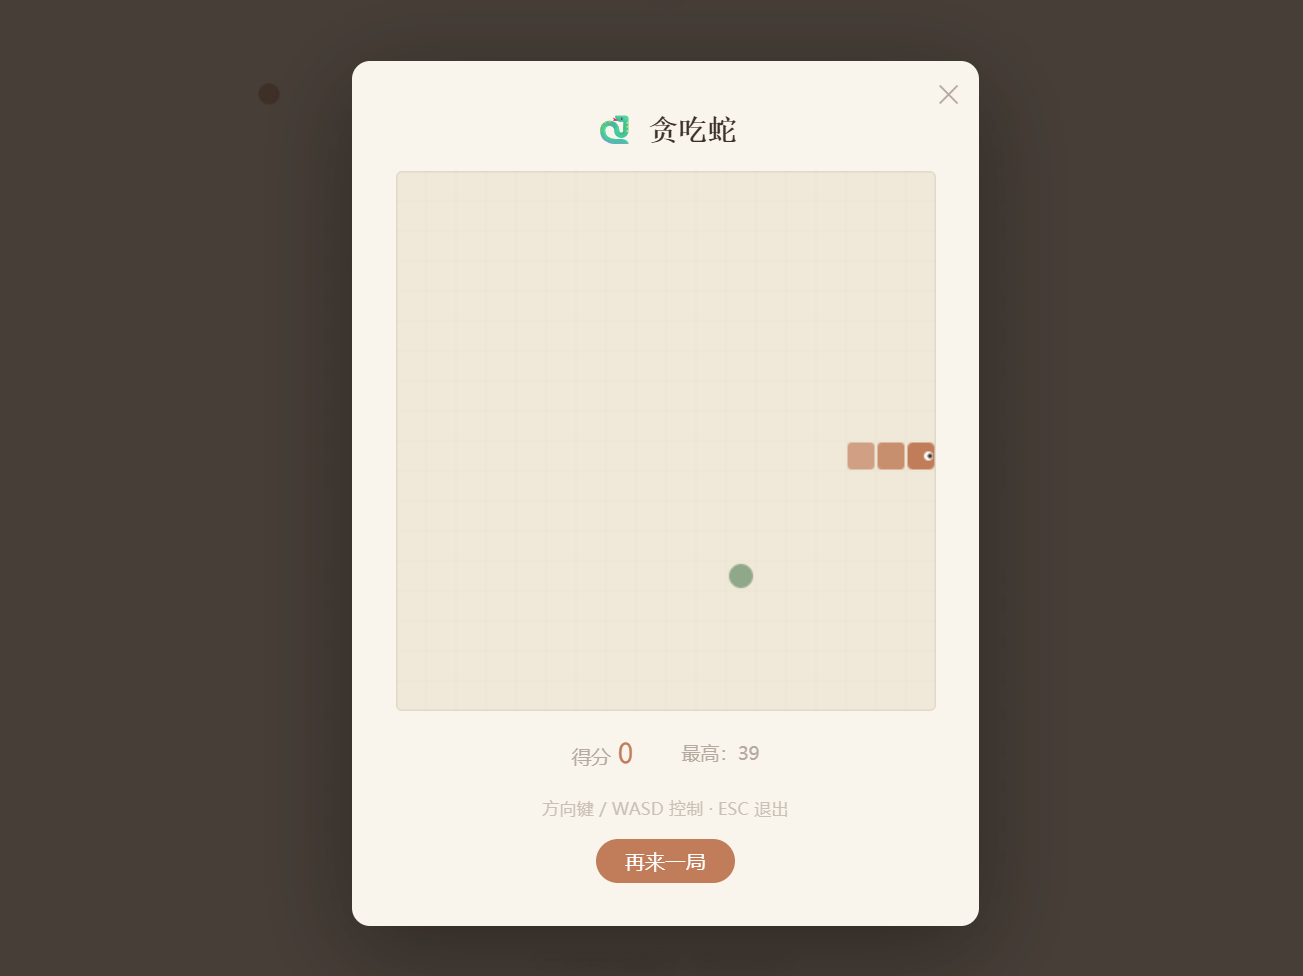
\includegraphics[width=0.85\linewidth]{../图片/贪吃蛇界面.png}
\caption{Hidden Snake mini-game: terra-cotta gradient snake body, sage green food, arrow keys or touch swipe control.}
\label{fig:snake}
\end{figure}

\subsection{Progressive Visual System Construction}

The visual system of Phase~2 did not emerge fully formed at the v1.0 stage. It evolved through three major versions and two rounds of visual enhancement:

\textbf{v1.0 (Foundation)} implemented the six-region structure, horizontal scroll interaction, and three footer easter eggs (time greeting, hidden playlist, hidden message), establishing a complete page skeleton. The visual style at this stage was intentionally restrained: warm cream background, serif headings, ample whitespace. Footer texture was limited to a single subtle CSS fiber grain layer.

\textbf{v1.1 (Experience and Visual Optimization)} incorporated multiple improvements after browser testing: a mobile degradation strategy (skipping horizontal scroll below 640\,px), region transition blending (chapter separator fade-in via IntersectionObserver), hero paper texture overlaid with four-corner vignette (via \texttt{radial-gradient}), a custom cursor (14\,px terra-cotta semi-transparent dot, enlarging to 28\,px when hovering interactive elements, with a footer toggle to disable), spotlight effect for Thought cards, article modal overlay and Notes lightbox, and a localStorage-based public message wall.

\textbf{v2.0 (Five-Module Upgrade)} systematically expanded both functionality and visuals: A---four independently themed data visualization panels; B---vitality system (14 Canvas particles drifting in the hero background, 4 plant SVGs enlarged to 120--160\,px with gentle sway animation, name breathing animation and tag pulsing); C---Snake game and achievement system; D---deep visual upgrade (staggered character drop entrance animation, hand-drawn decorative lines under section titles, five-level paper texture depth across regions, glow shifting between terra-cotta and amber on a 25-second cycle); E---atmosphere system with six time-of-day color transitions (checking every 30 seconds and smoothly updating \texttt{--bg} and related CSS properties).

\textbf{Two Rounds of Visual Enhancement.} After v2.0, two additional rounds of ``filling'' targeted visual sparseness. Round~1---Geometric Scaffolding: fixed side lines (1\,px gradient lines at 2.8\,rem from window edges), hero diamond decorative lines (horizontal gradient lines plus 45\textdegree\ diamond with 3.8\,s pulse), L-shaped corner frames for the About and Notes sections (30\,px, sage green, IntersectionObserver-triggered visibility), dot-decorated section titles, chapter separators upgraded to ``--- $\diamond$ ---'' (center diamond with 3-second pulse), geometric fold corners on all 12 cards (terra-cotta triangles for Thought cards, sage green triangles for Note cards, 4.5-second subtle flicker), a double-layer rotating dashed ring around the Contact social icons (inner ring 40\,s clockwise, outer ring 65\,s counterclockwise), a double-layer avatar border, a 30\,px dot-grid background pattern for the About section, and a $-7$\textdegree\ diagonal line texture for the Notes section. Round~2---Scrapbook Elements: 4 washi tape strips (CSS gradient simulation, diagonally placed at the edges of the About, Thoughts, Notes, and Message Wall sections), 3 ink stamps (a square ``collection'' stamp, a circular star stamp, a square ``read'' stamp), 4 hand-drawn line effects (highlight marker underlines for section titles, double-line borders for the interest tag group, an oval sketch around the avatar), 5 randomly rotated ($\pm7$\textdegree) paper scraps, 5 chapter page numbers (01--05), and an interactive peel-away sticker corner (rotating $-6$\textdegree\ on hover). All above decorations were implemented in pure CSS with zero additional image assets.

Notably, these five visual iterations (three major versions plus two rounds of enhancement) illustrate an important advantage of the Design-First strategy: \textbf{when the base skeleton is correct, adding decorative layers is remarkably efficient.} The scrapbook elements case is particularly telling---the user's prompt was a single sentence: ``Can the background keep a scrapbook feel while adding more elements?'' The AI proceeded to produce over 300 lines of CSS spanning six independent sub-schemes, because these decorative elements were entirely predictable within the aesthetic framework established by the design document---the AI knew what colors, what opacity levels, and what size ranges to use, requiring no additional directional calibration.

\subsection{Experience-Driven Iteration}

After the first implementation (v1.0) was completed, browser testing revealed several issues that could not have been detected at the design document level. Each of these was corrected through precise feedback prompts following a consistent structure---``describe what I saw + precisely describe the desired target behavior''---which proved far more efficient than vague ``fix this'' instructions:

\begin{itemize}
    \item \textbf{Back-to-top button invisible}: The button color blended into the footer background, making it nearly undiscoverable. Changed to a 40\,px circular button with a subtle border and hover highlight effect.
    \item \textbf{Navigation jumps jarring}: The top navigation and side dots used raw \texttt{href} jumps with no transition, clashing with the page's overall ``warm'' aesthetic. Changed to \texttt{window.scrollTo(\{behavior: `smooth'\})}.
    \item \textbf{Email icon behavior inappropriate}: The \texttt{mailto:} protocol had no effect on computers without a configured email client. Changed to clipboard copy with a Toast ``Copied'' notification.
    \item \textbf{Music icon SVG semantically wrong}: The QQ Music icon's SVG was actually a clock pattern (circle + hands). Replaced with a double eighth-note music symbol.
    \item \textbf{Card shine parameters off}: The shine effect was perpetually visible by default, with the brightness value (0.25) appearing harsh on actual screens. Changed to hover-triggered only, with brightness reduced to 0.14.
    \item \textbf{Interest tags lacked interaction cues}: The design assumed ``tags are clickable'' was obvious, but actual visitors did not know. Added a permanently visible ``Tap to explore $\rightarrow$'' text label to the left of the tag row.
\end{itemize}

\subsection{Strategy Comparison}

\begin{table}[t]
\centering
\caption{Qualitative comparison of the two Vibe Coding strategies.}
\label{tab:comparison}
\resizebox{\columnwidth}{!}{%
\begin{tabular}{p{0.45\columnwidth}p{0.45\columnwidth}}
\hline
\textbf{Incremental Build (Codex)} & \textbf{Design-First (Claude Code)} \\
\hline
Build skeleton $\rightarrow$ add modules one by one $\rightarrow$ adjust each & Discuss design $\rightarrow$ write design doc $\rightarrow$ implement against doc \\
\hline
No global design anchor; style direction unclear & Design document locks global direction, always controllable \\
\hline
Each module's outcome highly dependent on single-prompt precision & Design phase confirms direction; implementation phase has the document as reference \\
\hline
Correction direction vague, prone to drift & Document serves as correction anchor; modifications always grounded \\
\hline
Result: early stagnation, no complete deliverable & Result: complete homepage, deployed to production \\
\hline
\end{tabular}%
}
\end{table}

Table~\ref{tab:comparison} provides a qualitative comparison of the two strategies. It must be reiterated that, since the two strategies used different AI tools, there is some confounding between tool capability differences (e.g., Claude Code may excel in long-context dialogue maintenance and front-end code generation compared to Codex) and strategy effects---an inherent limitation of this experiment as a single-case study. Nevertheless, the experiential difference at the strategy level is clear: Incremental Build places the user in the dual role of ``designer plus debugger''---a role that a user without professional background can scarcely fulfill; Design-First transforms the user into a ``design reviewer''---a role that requires only aesthetic judgment (``does this look good?'') rather than professional knowledge (``what color palette should I use?'').

The most important lesson learned from this entire experiment is: \textbf{before asking the AI to write code, ask it to help with design.} The roughly 20\% upfront investment in design discussion paid for itself through sustained directional control, well-grounded corrections, and a final deliverable that far exceeded initial expectations.

\subsection{Implementation Statistics}

The final codebase consists of three files totaling approximately 3,700 lines: \texttt{index.html} (page structure, six semantic regions, approximately 470 lines), \texttt{style.css} (all styling, CSS custom properties, responsive breakpoints at 900\,px and 640\,px, approximately 3,100 lines), and \texttt{script.js} (GSAP-driven interactions including horizontal scroll, particle ecosystem, data panel theming, easter egg triggers, Snake game engine, time-based atmosphere switching, custom cursor logic, approximately 1,700 lines).
The asset directory includes an avatar image, six article cover images, Note section images (across four categories: Life, Gaming, Study, Materials), eight plant SVGs, two mp3 music files, and one pixel character spritesheet.
The site is deployed via GitHub Pages (URL: \url{https://qaq82625.github.io/-v2.0/}).
The complete dialogue comprised approximately 200+ rounds, covering design ideation, code implementation, and iterative refinement.
